% Matlab Implementation of Neural Field Model
% tex file of implementation document


\documentclass[a4paper, 12pt, english]{article}


% packages
\usepackage{amsmath}
\usepackage{graphicx}


% graphic path
\graphicspath{{/Users/miao/Documents/Miao/Neurosciences/Projects/NeuralFieldModel/Figures/}}


% title of this manuscript
\title{Matlab Implementation of Neural Field Model}
\author{Miao Cao}
\date{1 July 2016}


\begin{document}

% title of the document
\begin{titlepage}\centering
\vspace*{\fill}
\maketitle
\vspace*{\fill}
\end{titlepage}

\tableofcontents

\newpage



% Introduction
\section{Introduction}
\paragraph{In order to implement and simulate Neural Field Model, we break down
the model into several parts and implement and test each of them independently. The
following sections show the details of our implementation. Please always refer to
Freestone et al., 2011, NeuroImage to equations and details.}

\newpage




% Convolution of two Gaussians
\section{Convolution of Two Gaussian Basis Functions}

\paragraph{Analytically prove convolution of two Gaussians. In general, the
precision level of analytic simulation should be around $10^{-6}$.}

\paragraph{File (Matlab script): Convolution2DGaussians.m}

\subsection*{Matlab script description}

Appendix E (Freestone et al., 2011, NeuroImage), Equation (4) $\left(\phi_{i}\otimes\phi_{j}\right)(r)=(\frac{\pi\sigma_{i}^{2}\sigma_{j}^{2}}{\sigma_{i}^{2}+\sigma_{i}^{2}})^{\frac{n}{2}}\exp(-\frac{1}{\sigma_{i}^{2}+\sigma_{i}^{2}}r^{T}r)$.

\subparagraph{Section: Generate spatial data, create a $NPoints\times NPoints$ cortical surface and phi and psi Gaussian basis functions.\\}


\begin{tabular}{|c|c|}
\hline
Variable name & Explanation\tabularnewline
\hline
X & Coordinates of x-axis\tabularnewline
\hline
Y & Coordinates of y-axis\tabularnewline
\hline
mu\_phi & Centre of gaussian\tabularnewline
\hline
sigma\_phi & covariance matrix of phi\tabularnewline
\hline
phi & Gaussian basis function\tabularnewline
\hline
mu\_psi & Centre of gaussian\tabularnewline
\hline
sigma\_psi & covariance matrix of psi\tabularnewline
\hline
psi & Gaussian basis function\tabularnewline
\hline
\end{tabular}

\paragraph{Analytic check of convolution of two Gaussians.\\}
\label{subp:Analytic check of convolution of two Gaussians}

%\subparagraph{Section: analytic check of convolution of two gaussians}

\begin{tabular}{|c|c|}
\hline
Variable name & Explanation\tabularnewline
\hline
mu & Centre of a gaussian resulted from convolution of two gaussians, phi
and psi\tabularnewline
\hline
var\_phi & variance of gaussian phi\tabularnewline
\hline
var\_psi & variance of gaussian psi\tabularnewline
\hline
exponential & exponential part of Equation Appendix E.4 (Freestone et al. 2011)\tabularnewline
\hline
CovMat & covariance matrix of a resultant gaussian convolved by two other gaussians\tabularnewline
\hline
coefficient & coefficient part of Equation Appendix E.4 (Freestone et al. 2011)\tabularnewline
\hline
convE2\_equivalent & analytic result of convolution of two gaussians, phi and psi\tabularnewline
\hline
\end{tabular}

\newpage




% Compute Gamma
\section{Compute Gamma}

\paragraph{File (Matlab script): ComputeGamma.m}

\subsection*{Matlab script description}

\paragraph{This matlab script mainly implement and estimate the following two
equations, (21) and Appendix (D.7) (Freestone et al. 2011 NeuroImage).}

\paragraph{Field, v(r), is decomposed of a finite-dimensional state vector and
a vector of Gaussian basis functions.}

\paragraph{Define $\Gamma=\int_{\Omega}\phi(r)\phi^{T}(r)dr$. Firstly, programmatically
define $\phi(r)$, as a vector of Gaussian basis functions. Each Gaussian
function is defined as $\phi(r-r')=\exp{(-\frac{(r-r')^{T}(r-r')}{\sigma_{\phi}^{2}})}$.}

\newpage



% Compute Psi
\section{Compute Psi}
We implement to compute Psi.

\[[\Psi(r\prime)] = Ts\Gamma\int_\omega\]


\newpage


\section{Compute State Vector at time T+1}
\label{state vector}
\paragraph{parameter table, figures}

\newpage





\section{Compute Reduced Model}

\newpage





\section{Compute Full Model}
\paragraph{We compute the full model.}

\newpage


\section{Compare Reduced Model and Full Model}
Compare reduced model and full model.
\begin{figure}
\centering
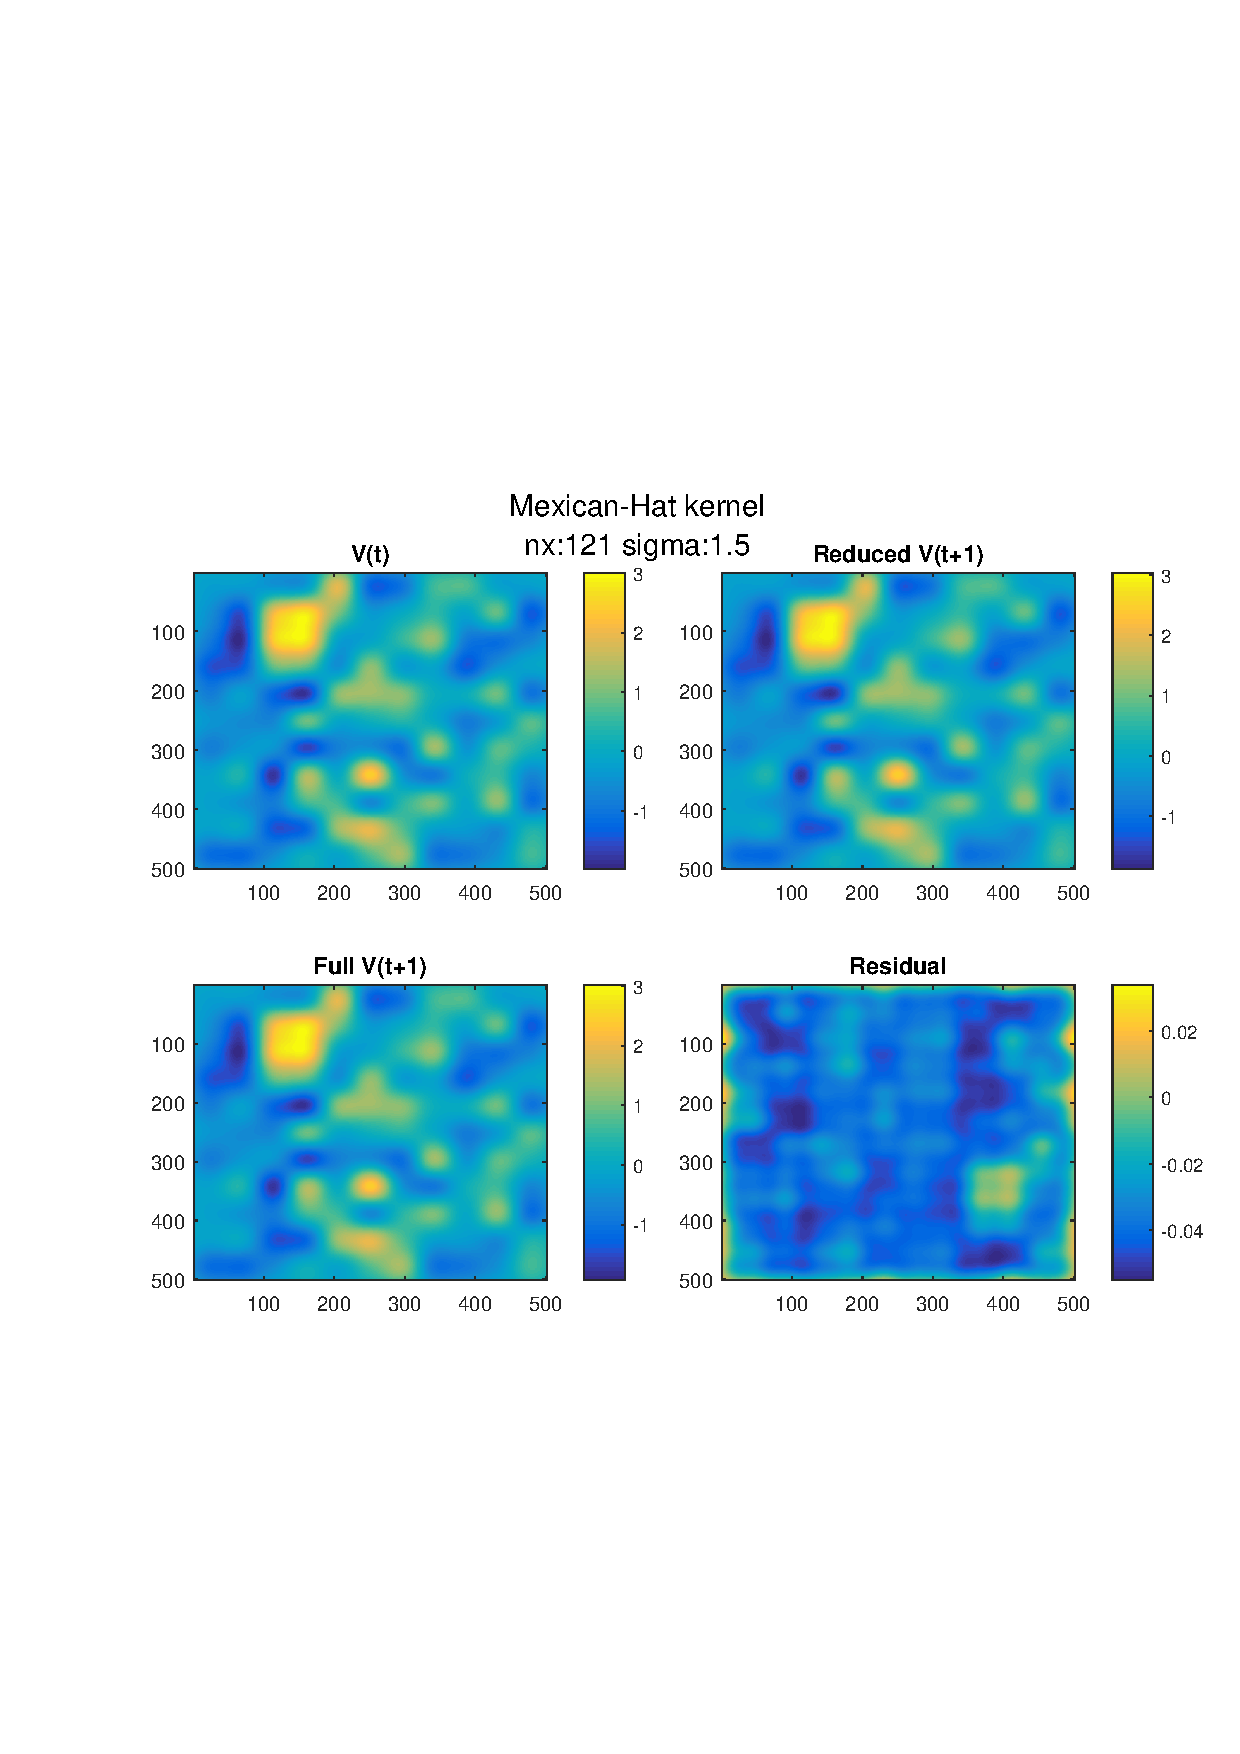
\includegraphics[width=0.8\textwidth]{modelComparison_MexHat_nx_121_sigma_1_5_nPoints_501_vTPlus1.pdf}
\caption{Connectivity kernel, Mexican Hat}
\end{figure}


\end{document}
